\documentclass[11pt]{article}
\usepackage[final]{acl}
\usepackage{times}
\usepackage{latexsym}
\usepackage[T1]{fontenc}
\usepackage[utf8]{inputenc}
\usepackage{microtype}
\usepackage{inconsolata}
\usepackage{graphicx}
\usepackage{booktabs}
\usepackage{amsmath}
\usepackage{placeins}
\graphicspath{{../results/figures/}}
\renewcommand{\topfraction}{0.9}
\renewcommand{\bottomfraction}{0.8}
\renewcommand{\textfraction}{0.07}
\renewcommand{\floatpagefraction}{0.75}
\setcounter{topnumber}{3}
\setcounter{bottomnumber}{2}
\setcounter{totalnumber}{5}

\newcommand{\fig}[1]{Figure~\ref{fig:#1}}

\title{Who Does a CV Screener Pass On?\\
An Explainable-AI Audit of Gender Bias in Occupation Classification}

\author{mangelv011 \\
  \texttt{https://github.com/mangelv011/hiring-bias-xai}}

\begin{document}
\maketitle

\begin{abstract}
A recruiter searches for a surgeon, and an AI model decides which candidate bios reach them. I audit such a screener: DeBERTa-v3-small fine-tuned to read a short professional bio and label which of 28 jobs it describes, trained on Bias in Bios. Of 100 qualified surgeons it passes on 76 men but 56 women, and over all 28 jobs it favours the majority gender of each job, more so the larger that majority is ($r = 0.85$). I then ask why, with explainable-AI methods that check one another. Shapley values and an exact decomposition of the score gap show that pronouns alone put women surgeons 1.1 log-odds below men, and that the strongest single word in the largest gap is the name of a website found only in women's bios. Swapping pronouns changes few decisions beyond what any edit does, deletion curves confirm that the top words matter while their order depends on the method, and probing and patching show gender left inside the model after the pronouns are gone. Removing pronouns narrows the gap by 20\% for half a point of macro-F1. A black-box audit of a local LLM screener finds no gap between women's and men's names. All code, results and figures are public.
\end{abstract}

\section{Introduction}

Employers screen candidates with models that read text. In the setting I study, a model reads each candidate's short professional bio and decides which of 28 jobs it describes; a recruiter searching for ``surgeon'' sees the bios labelled surgeon and never sees the rest. A candidate is \emph{qualified} for a search when the bio belongs to someone who really does that job. A fair screener passes on the same share of qualified women and qualified men: equal true positive rates, or equal opportunity \citep{hardt2016equality}.

Such a system is high-risk under the EU AI Act \citep[Annex III]{euaiact2024}: the provider has to show that the ranking does not depend on gender and, if it does, why. Accuracy cannot answer that. The stakeholders are the candidates, who are passed over without knowing it; the recruiter, who sees a biased shortlist; and the platform, which carries the legal duty.

\citet{dearteaga2019bias} showed that occupation classifiers on these bios reproduce the gender imbalance of each job. I repeat that measurement on a modern transformer and go further, asking four questions with methods chosen so that each checks another: \emph{why} the model decides as it does (Shapley attribution and an exact gap decomposition), whether the explanation can be \emph{trusted} (counterfactual swaps, deletion curves and stability checks), \emph{where} gender lives inside the model (probing and activation patching), and \emph{what fixes it} at what cost. Last, I audit a general-purpose LLM used as a screener, where only inputs and outputs can be observed.

\section{Data and Methods}

\paragraph{Data.} Bias in Bios \citep{dearteaga2019bias}, in the release of \citet{ravfogel2020inlp} \citep{ravfogel2020biasbios}, pinned to one revision. The first sentence of each bio, which names the title, is removed, so the model has to infer the job from the rest. Gender was inferred by the dataset authors from the pronouns, and is binary. I train on a stratified subsample of 60,000 bios, select on 10,000 and test on all 99,069 test bios. The share of women ranges from 9\% (rapper) to 93\% (dietitian). For the explanation work I use a \emph{showcase subset} of 1,721 test bios: among jobs with at least 500 test bios, the three with the most women (dietitian, nurse, model) and the three with the fewest (surgeon, software engineer, composer), up to 150 women and 150 men each.

\paragraph{Models.} The \emph{main model} is DeBERTa-v3-small \citep{he2023debertav3} fine-tuned for five epochs (learning rate $3\times10^{-5}$, chosen on dev, seed 42). The \emph{baseline model} is TF-IDF on 1--2 grams with logistic regression. A bio's \emph{score} for a job is its log-odds; every explanation below explains that score.

\paragraph{Measuring bias.} For each job, the \emph{gap} is the share of qualified women passed on minus the share of qualified men (the TPR gap). The overall gap is its root mean square over jobs \citep{romanov2019name}. All intervals are 95\% bootstrap intervals over bios. To check that gaps are not luck, I shuffle gender within each job 1,000 times; per-job tests use the Holm correction \citep{holm1979simple}.

\paragraph{Explanation methods.} Each method answers one question; Table~\ref{tab:methods} says why each fits.

\emph{Shapley attribution} splits a bio's score among its words \citep{shapley1953value,lundberg2017unified}, estimated with 40 random word orders per bio, each also read backwards \citep{strumbelj2014explaining}. An absent word is deleted, so the model never sees a placeholder it was not trained on. I use it because its parts add up exactly to the score, which the next method needs.

The \emph{gap decomposition} adds Shapley values over bios: the gap between women's and men's average score for a job splits exactly into one part per word. It tells how the gap is made up, not what an edit would do.

\emph{Counterfactual swaps} exchange gendered words (\emph{he}$\leftrightarrow$\emph{she}, \emph{Mr}$\leftrightarrow$\emph{Ms}) with a part-of-speech tagger to resolve \emph{her} \citep{kusner2017counterfactual}. Any edit can flip a borderline decision, so each swap has a control that deletes the same words.

\emph{Deletion curves} remove words in order of attribution (MoRF), in reverse (LeRF) and at random, replacing them with \texttt{[UNK]} so the check does not repeat how the values were made \citep{samek2017evaluating}. \emph{Stability} compares the ranking with another seed, with \texttt{[UNK]} instead of deletion, and with leave-one-out.

A linear \emph{probe} \citep{belinkov2022probing} tries to read gender from each layer of bios with pronouns and titles removed, against the gender predicted from the job alone and against probes on shuffled labels \citep{hewitt2019designing}. \emph{Activation patching} \citep{meng2022locating,heimersheim2024patching} copies the states of the original bio into the run on its swap, at one layer and one set of positions, and measures how much of the original score comes back.

\begin{table}[!tbp]
\small
\begin{tabular}{@{}p{0.27\columnwidth}p{0.66\columnwidth}@{}}
\toprule
Method & Why it fits here \\
\midrule
Shapley & Model-agnostic and exactly additive, so word parts can be summed over bios. \\
Gap decomposition & Turns per-bio values into the part of the women--men gap each word makes. \\
Swaps & Tests causation, which attributions cannot; the deletion control separates gender from editing. \\
Deletion curves & Checks that high values point at words the model needs. \\
Probing & Asks if gender is still readable after scrubbing. \\
Patching & Asks where the swap's effect sits, layer by layer. \\
Name audit & The only option for an LLM seen as a black box. \\
\bottomrule
\end{tabular}
\caption{Methods and the reason for each.}
\label{tab:methods}
\end{table}

\paragraph{Mitigation.} I retrain the main model on bios with pronouns and titles removed (the \emph{scrubbed model}, same recipe), and separately delete \emph{proxy words}. These are words that are not gendered but that the gender the gap favours uses at least three times as often, in at least 5\% of its bios, and whose part of the gap points the same way as the pronouns'. I fixed this rule before the evaluation, after correcting a first version that picked function words such as \emph{the}; the correction is recorded in the repository.

\paragraph{LLM audit.} Ternary Bonsai 2 9B \citep{prismml2026bonsai}, a 2-bit version of Qwen3.5-9B, served locally (temperature 0, thinking off). It reads a job ad and a bio and answers JSON with a reason, then yes or no. Each of 600 profiles (100 per showcase job, 70 qualified) is shown with no header, a neutral ID line, swapped pronouns, or a name from one of four origin groups and both genders, with pronouns matching the name. Names are the most frequent in Spain's statistics \citep{ine2025names}, following \citet{bertrand2004emily} and recent LLM audits \citep{salinas2024name,wen2025faire}. A manipulation check first asks the model where each bare name comes from; identical reruns and a whitespace edit give the noise floor.

\section{Results}

\paragraph{Performance.} The main model gives the right job for 83.7 of 100 test bios (macro-F1 0.783 [0.779, 0.788]), the baseline model for 79.5 (0.728 [0.724, 0.733]). Its overall gap is lower (0.148 against 0.167) but the intervals overlap: the more accurate model is not clearly fairer.

\begin{figure}[!tbp]
\centering
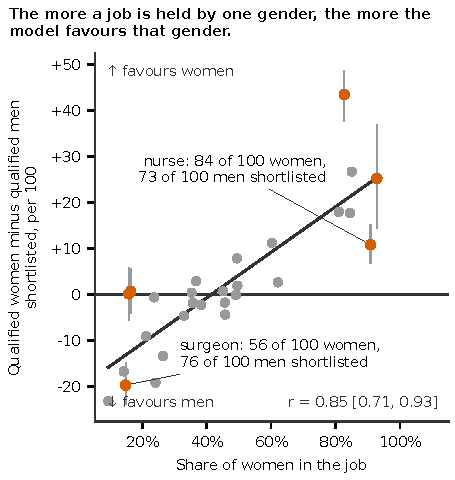
\includegraphics[width=\columnwidth]{f1_gap_vs_share.pdf}
\caption{Each dot is a job, with its 95\% interval. Above 0 the model passes on more qualified women than men, per 100 of each.}
\label{fig:f1}
\end{figure}

\paragraph{The gap follows the share of women (\fig{f1}).} Of 100 qualified surgeons the main model passes on 56 women and 76 men; of 100 nurses, 84 women and 73 men. Over the 28 jobs the gap rises with the share of women ($r = 0.85$ [0.71, 0.93]) and stays between 0.84 and 0.87 when any one job is left out. Shuffled genders never produced an overall gap as large ($p \le 0.001$). Ten jobs have a gap clearly different from zero after the Holm correction; in the other 18 the data cannot tell it from zero.

\begin{figure}[!tbp]
\centering
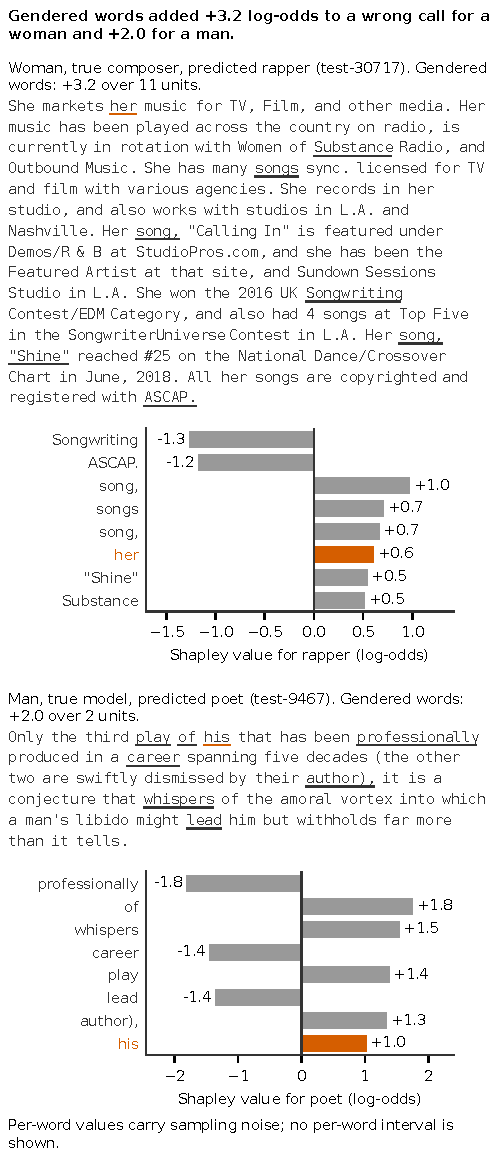
\includegraphics[width=\columnwidth]{f2_shapley_cases.pdf}
\caption{Two wrong decisions and the words that moved them, chosen by a rule fixed before looking. Gender words are highlighted.}
\label{fig:f2}
\end{figure}

\paragraph{Single decisions (\fig{f2}).} A woman composer labelled rapper: her 11 gender words add +3.2 log-odds to ``rapper''. A man who works as a model, labelled poet: his 2 gender words add +2.0 to ``poet''. In both, the strongest words are about the work. These are the most extreme of 114 and 154 wrong decisions, so they illustrate the mechanism and are not typical.

\begin{figure}[!tbp]
\centering
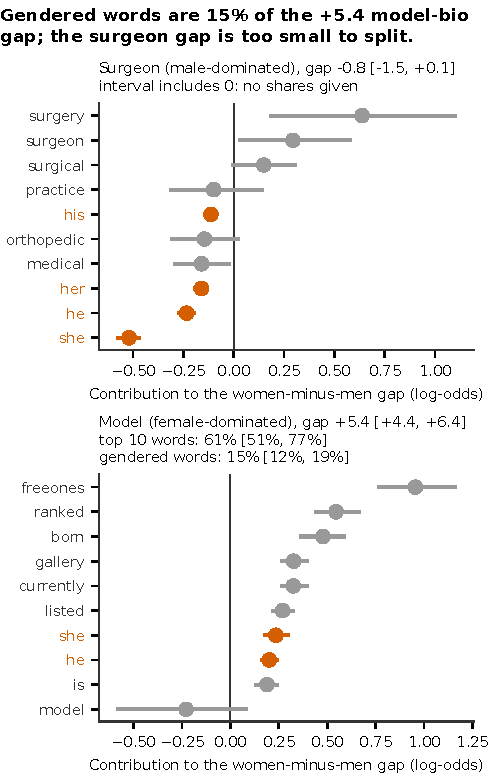
\includegraphics[width=\columnwidth]{f3_gap_words.pdf}
\caption{The ten words that make up most of the score gap between women and men, with 95\% intervals. Gender words are highlighted.}
\label{fig:f3}
\end{figure}

\paragraph{What makes up the gap (\fig{f3}).} In surgeon bios the overall score gap ($-0.77$ [$-1.54$, $+0.08$]) cannot be told from zero, yet the gender words alone put women 1.12 [1.02, 1.24] log-odds below men, while words about the job pull the other way. In nurse bios gender words favour women by 1.97. In \emph{model} bios, women score 5.40 higher; gender words make up only 15\% of that. The strongest single word is \texttt{freeones}, the name of a website listing adult performers: it appears in 54 of 150 women's bios and none of 150 men's. Part of this gap comes from where some bios were published, not from pronouns. The baseline model shows the same signs in every job.

\begin{figure}[!tbp]
\centering
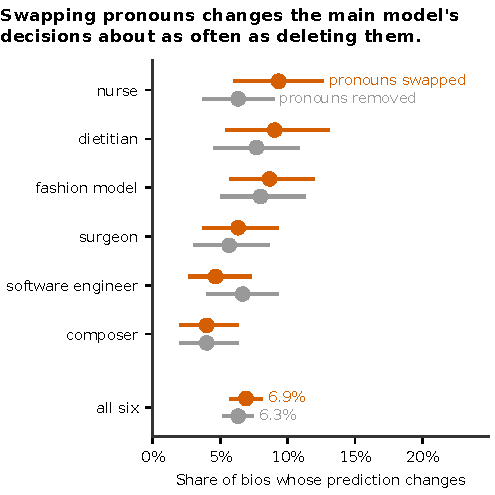
\includegraphics[width=\columnwidth]{f4_flip_rates.pdf}
\caption{Share of decisions that change when pronouns are swapped (highlight) or deleted (grey), main model, with 95\% intervals.}
\label{fig:f4}
\end{figure}

\paragraph{Does changing only the gender change the decision? (\fig{f4})} Swapping changes 6.9\% [5.7, 8.1] of the main model's decisions and deleting the same words changes 6.3\% [5.2, 7.5]: most flips come from editing the text. Yet when a swap does flip a decision, 88\% of the time the new job is held more by the new gender, against 72\% for deletions, so the flips lean towards gender stereotypes. The baseline model reacts more to the swap itself (13.5\% against 8.8\%). Reading 50 swapped bios by hand, 3 read wrongly.

\begin{figure}[!tbp]
\centering
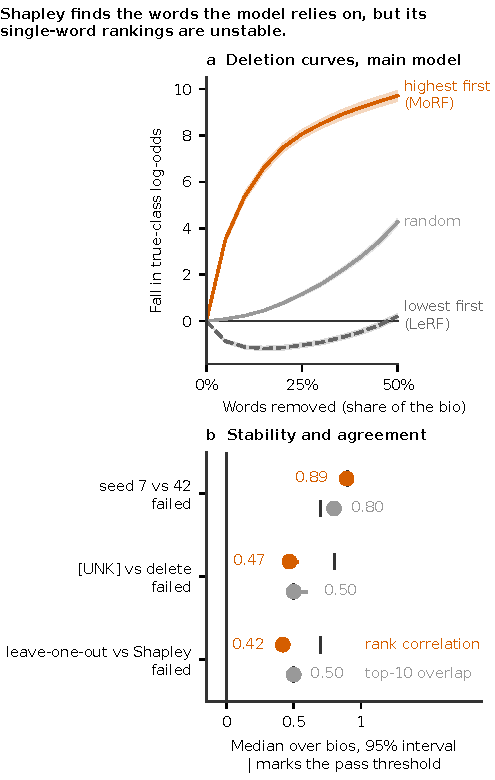
\includegraphics[width=\columnwidth]{f5_explanation_checks.pdf}
\caption{(a) Fall in the true job's score as words are removed in three orders. (b) Agreement of the main ranking with three alternatives.}
\label{fig:f5}
\end{figure}

\paragraph{Can the explanations be trusted? (\fig{f5})} Removing words with the highest Shapley values first lowers the main model's score by 7.0 log-odds on average, against 1.5 at random and a rise of 0.7 for the lowest first: the values point at words the model needs. Two Shapley runs with different seeds rank a bio's words almost the same way (median rank correlation 0.89, 8 of the top 10 shared). Hiding a word with \texttt{[UNK]} instead of deleting it (0.47), or using leave-one-out (0.42), changes the order far more. In one surgeon bio, \emph{practice} and \emph{practices} each appear twice: Shapley shares their credit, while leave-one-out gives each almost nothing because the others carry the same information. The totals over many bios (\fig{f3}) are the solid result; single-bio rankings (\fig{f2}) are indications.

\begin{figure}[!tbp]
\centering
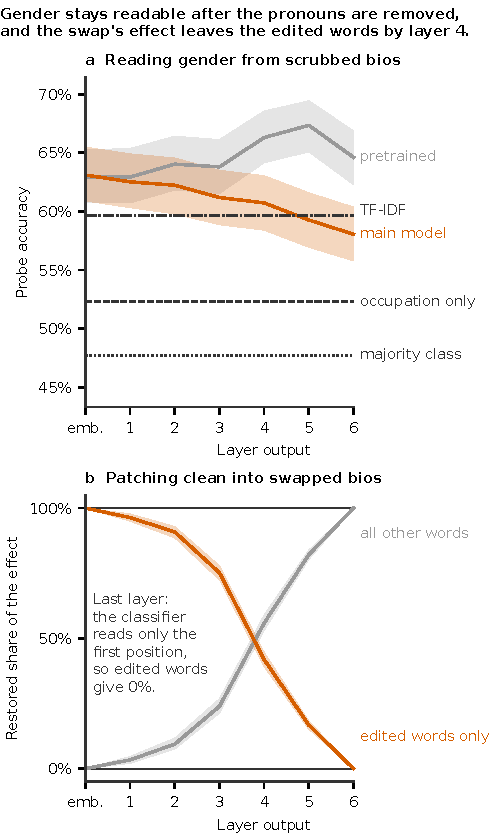
\includegraphics[width=\columnwidth]{f6_probing_patching.pdf}
\caption{(a) Probe accuracy for gender on bios without pronouns, by layer. (b) Share of the swap's effect restored by patching the swapped words or the other words.}
\label{fig:f6}
\end{figure}

\paragraph{Gender inside the model (\fig{f6}).} On bios without pronouns or titles, a probe still guesses gender 63\% of the time from the main model's embeddings and 58\% from its last layer, against 52.3\% from the job alone and 59.7\% from TF-IDF on the same words. Names, topics and site names carry it. Fine-tuning makes it a little harder to read in the last layers. Patching 168 bios that the swap moves most, the swapped words alone restore 96\% of the effect at layer 1, 42\% at layer 4 and 17\% at layer 5, while all the other words restore 3\%, 56\% and 82\%. Attention carries the gender signal away from the pronouns within four layers. A fix that edits only pronoun positions would have to act early.

\section{Actions and Insights}

\begin{figure}[!tbp]
\centering
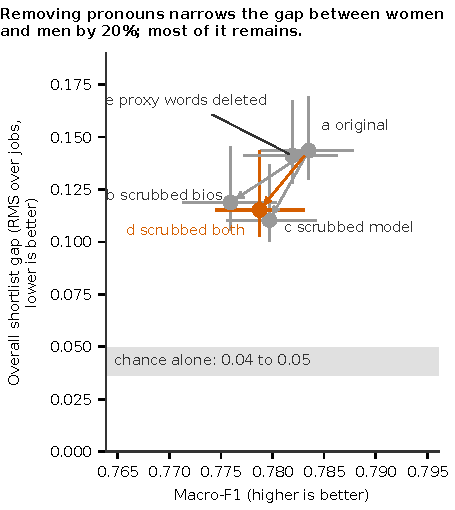
\includegraphics[width=\columnwidth]{f7_mitigation.pdf}
\caption{Each condition's macro-F1 against its overall gender gap, with 95\% intervals; the grey band is what shuffled genders give.}
\label{fig:f7}
\end{figure}

\begin{table}[!tbp]
\small
\centering
\begin{tabular}{@{}lccc@{}}
\toprule
Condition & Macro-F1 & Gap & Change in gap \\
\midrule
a. original & 0.784 & 0.143 & \\
b. scrubbed bios & 0.776 & 0.119 & $-0.025$ \\
c. scrubbed model & 0.780 & 0.110 & $-0.033$ \\
d. scrubbed both & 0.779 & 0.115 & $-0.028$ \\
e. proxy words out & 0.782 & 0.141 & $-0.002$ \\
\bottomrule
\end{tabular}
\caption{Mitigation on 97,348 test bios outside the showcase subset. The change is paired with (a); its interval excludes 0 for b--d and includes 0 for e.}
\label{tab:mitigation}
\end{table}

\paragraph{What removing the cues achieves (\fig{f7}, Table~\ref{tab:mitigation}).} Training and scoring on bios without pronouns (d) lowers the overall gap from 0.143 to 0.115, a 20\% cut, for 0.5 points of macro-F1. Scrubbing only the bios at scoring time (b) does almost as much with no retraining. Deleting the six proxy words leaves the gap where it was. The remaining gap is still more than twice what chance gives (0.050). By job, the gap in \emph{model} moves from 44 to 40 more qualified women than men passed on per 100, and in surgeon from 22 to 18 fewer women.

\paragraph{Recommendations to the platform.} (1)~Scrub pronouns and titles both in training and at scoring time: it is cheap and does part of the work. (2)~Do not stop there or claim the screener is fair: the gap that remains sits in other words and in the model's states (\fig{f6}), so the next step is to remove gender from the representation itself \citep{ravfogel2020inlp,belrose2023leace}. (3)~Measure the gap per job, with intervals, on every new model before it is used, because the overall number hides jobs such as \emph{model} and surgeon. (4)~Read explanations as totals over many bios, never word by word for one candidate.

\paragraph{An LLM screener.} The model read the gender of 372 of 375 names and recognised Moroccan, Romanian and British names, but took most Spanish names for Hispanic American; I merged those two groups, as fixed in advance. Table~\ref{tab:llm} gives the results. With a woman's or a man's name it says yes to 53 of 100 qualified candidates either way: the difference is $-0.5$ points [$-4.7$, $+3.5$], so gaps of 5 points or more are ruled out. No origin group differs from the British one after Holm. Having any name at all lowers the yes-rate by 6.0 points [2.1, 10.1], a comparison I had not planned and read as a lead. Rewording the instruction moves it more (59 to 47 or 39). Of 594 changed decisions, 85\% give a reason that does not mention name, origin or gender; about four in ten of those changes would also follow a whitespace edit.

\begin{table}[!tbp]
\small
\centering
\begin{tabular}{@{}lc@{}}
\toprule
Presentation of the bio & Yes, of 100 qualified \\
\midrule
No header & 59 [55, 64] \\
Neutral ID line & 61 \\
Pronouns swapped & 57 \\
Woman's name (four groups) & 53 \\
Man's name (four groups) & 53 \\
\midrule
Origin vs.\ United Kingdom & change, points \\
\quad Morocco & $+1.5$ [$-5.3$, $+9.1$] \\
\quad Romania & $0.0$ [$-7.8$, $+7.8$] \\
\quad Spain + Hispanic America & $+3.0$ [$-4.1$, $+9.3$] \\
\bottomrule
\end{tabular}
\caption{LLM screener on 600 profiles (8,167 calls, 3.0 hours on the laptop).}
\label{tab:llm}
\end{table}

\begin{figure}[!tbp]
\centering
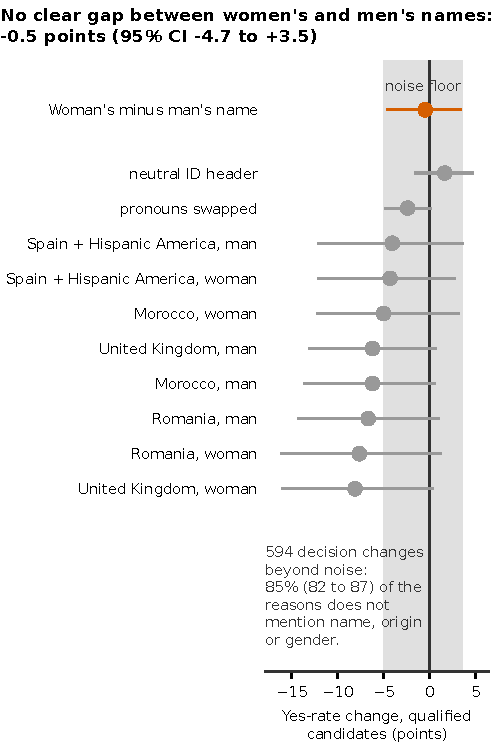
\includegraphics[width=\columnwidth]{f8_llm_screener.pdf}
\caption{Change in yes per 100 qualified candidates against no name, with 95\% intervals and the noise floor (grey).}
\label{fig:f8}
\end{figure}

\section{Discussion}

\paragraph{Where the methods agree and disagree.} Attribution, swaps and probing agree that gender words push decisions towards the majority gender of each job, and that removing them leaves gender readable. They disagree on how much the pronouns matter: in F3 they make up a large part of the surgeon and nurse gaps, yet swapping them flips few decisions beyond an edit (F4). The two are compatible. A decomposition measures how the score is made up, while a swap only flips decisions near the boundary. They are still a warning against reading attribution as causation \citep{jacovi2020faithfully}.

\paragraph{How explanations could mislead a stakeholder.} A recruiter shown F2 might conclude that the model ``uses gender'' for that candidate; the word ranking of one bio changes with the method (F5), so that reading is fragile. A compliance team shown that pronouns were removed might conclude that gender is gone; F6 shows it is not. The \texttt{freeones} finding is easy to misread as a fact about women; it is a fact about where some bios were collected.

\paragraph{Limitations.} One training run per model, so the scrubbed and original models differ also by run-to-run noise. Gender is binary and inferred from pronouns. The deletion check uses \texttt{[UNK]} for a model trained on deletion; retraining-based evaluation \citep{hooker2019benchmark} was too costly, and weight randomization \citep{adebayo2018sanity} would pass by construction for a black-box method. Patching shows that the swapped words' states are sufficient to restore the effect, not that they are necessary. The LLM audit covers one small model, one prompt with two rewordings and six jobs; companies use larger models, and the code accepts any OpenAI-compatible server. Its stated reasons were labelled by one reader. Stated reasons of LLMs need not reflect their computation \citep{turpin2023language}.

\paragraph{Future work.} Remove gender from the representation with LEACE or INLP and measure the gap and its cost the same way; repeat the LLM audit on larger models and in Spanish; add non-binary and name-based signals to the bios.

\FloatBarrier
\section*{Reproducibility}
Code, pinned data revision, result files, figures, decision records and a notebook that reads every number are at \url{https://github.com/mangelv011/hiring-bias-xai}. All experiments ran on one laptop with a 4 GB RTX 3050 GPU.

\bibliography{references}

\end{document}
